\usetikzlibrary{positioning,arrows,calc}

\tikzset{
modal/.style={>=stealth’,shorten >=1pt,shorten <=1pt,auto,node distance=1.5cm,
semithick},
world/.style={circle,draw,minimum size=0.7cm,fill=gray!15},
point/.style={circle,draw,inner sep=0.5mm,fill=black},
reflexive above/.style={->,loop,looseness=7,in=120,out=60},
reflexive below/.style={->,loop,looseness=7,in=240,out=300},
reflexive left/.style={->,loop,looseness=7,in=150,out=210},
reflexive right/.style={->,loop,looseness=7,in=30,out=330}
}

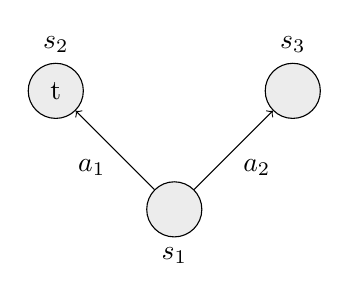
\begin{tikzpicture}[x=1.cm, y=1.cm]

\node[world] (s1) [label=below:$s_1$] {};
\node[world] (s2) [label=above:$s_2$,above left=of s1] {t};
\node[world] (s3) [label=above:$s_3$,above right=of s1] {};



\path[->] (s1) edge node[below left] {$a_1$} (s2);
\path[->] (s1) edge node[below right] {$a_2$} (s3);

\end{tikzpicture}